https://www.overleaf.com/project/5e945e8e5cc9d70001c66f9d


\documentclass{article}
\usepackage[utf8]{inputenc}
\usepackage{graphicx}
\usepackage{lipsum}
\usepackage{float}
\usepackage[margin=1in,left=1.5in,includefoot]{geometry}

% Header and Footer
\usepackage{fancyhdr}
\pagestyle{fancy}
\fancyhead{}
\fancyfoot{}
\fancyfoot[R]{ \thepage\ }
\renewcommand{\footrulewidth}{0pt}
%


\begin{document}

% title page content
\begin{titlepage}
    \begin{center}
        
\includegraphics[height= 4cm ]{UoRlogo.png} \\
        [5mm]
        \textsc{\Large University of Reading} \\
        [0.5cm]
        \textsc{\Large Department of Computer Science} \\
        [1cm]

        \line(1,0){300}\\
        [0.25in]
        \huge{\bfseries Extending a Platform Game in C/CC++: User Experience Enhancement}\\
        [2mm]
        \line(1,0){200} \\
        [1cm]
        \textsc{\Large Jason Jay Dookarun} \\
        [2mm]
        \textsc{\large Word Count: TBC} \\
        [2mm]
        \textsc{\large Page Count: 6}\\
        [4cm]
        \end{center}
        \begin{flushright}
        \textsc{\normalsize Module Code: CS1PR16 \\
        Student Number: 26017434 \\
        Time Spent: 50 Hours \\
        April 21, 2020 } \\
        \end{flushright}
\end{titlepage}

% front matter
\pagenumbering{roman}
\section*{Summary}
\addcontentsline{toc}{section}{\numberline{}Summary}

The following document consists of an in-depth systematic examination of elements developed by Jason Jay Dookarun to an existing C/C++ program developed by Parallel Realities. The given program is a platform game that employs the SDL2 library for the demonstration of graphics. A feature has been composed, modified and extended, integrated within the provided game, with the support provided by the skeleton code, authorised by \textbf{Dr Julian Krunkel} of the Department of Computer Science at the University of Reading. The aforementioned will further elaborate on the procedures undertaken to develop the feature(s) including design illustrations, methods of implementation and development process.
%\cleardoublepage

\section*{Declaration}
\addcontentsline{toc}{section}{\numberline{}Declaration}

I, \textbf{Jason Jay Dookarun}, of the Department of Computer Science at the University of Reading, confirms that all the sentences, figures, tables, equations, code snippets, artwork and illustrations in this report are original and have not been taken from any other person’s work, except where the works of others have been explicitly acknowledged, quoted and referenced. I understand that if failing to do so will be considered as a case of plagiarism. Plagiarism is a form of academic misconduct and will be penalised accordingly.

    \begin{flushright}
    \textbf{Jason Jay Dookarun} \\
    April 21, 2020\\
    [2cm]
    \end{flushright}

\rhead{Declaration}
\tableofcontents
\thispagestyle{empty}
\cleardoublepage






\newpage
\section{Introduction}\label{sec:intro}
\rhead{Introduction}
\lhead{Extending a Program in C/C++}
The provided program employs an SDL2 library to illustrate graphical components, coded in C/C++. This program has been developed and created by Parallel Realities. This project aims to develop an extension to the existing piece and further describe the choice made and implementation cycle applied. Authorised by the academic staff members at the University of Reading, I was provided with a skeleton code containing sections of the existing platform game, namely "Pete's Pizza Party 6".

The aim of the game entails accumulating all objects positioned across disparate seconds of the map. These objects would be portrayed as pizza slices. As the user assembled every pizza slice, the HUD, located on the right-hand side of the user's screen, would increment, accordingly. Once the entity collected all the elements, the game would be terminated.

To understand the game and existing mechanisms implemented, my first initiative involved executing the program. This allowed me the remark sectors of the program that could be: added, improved or modified. Moreover, by applying such, I would then be able to understand what sections of the game could be either improved or added, by using previous knowledge of gaming.
\begin{figure}[H]
    \centering
    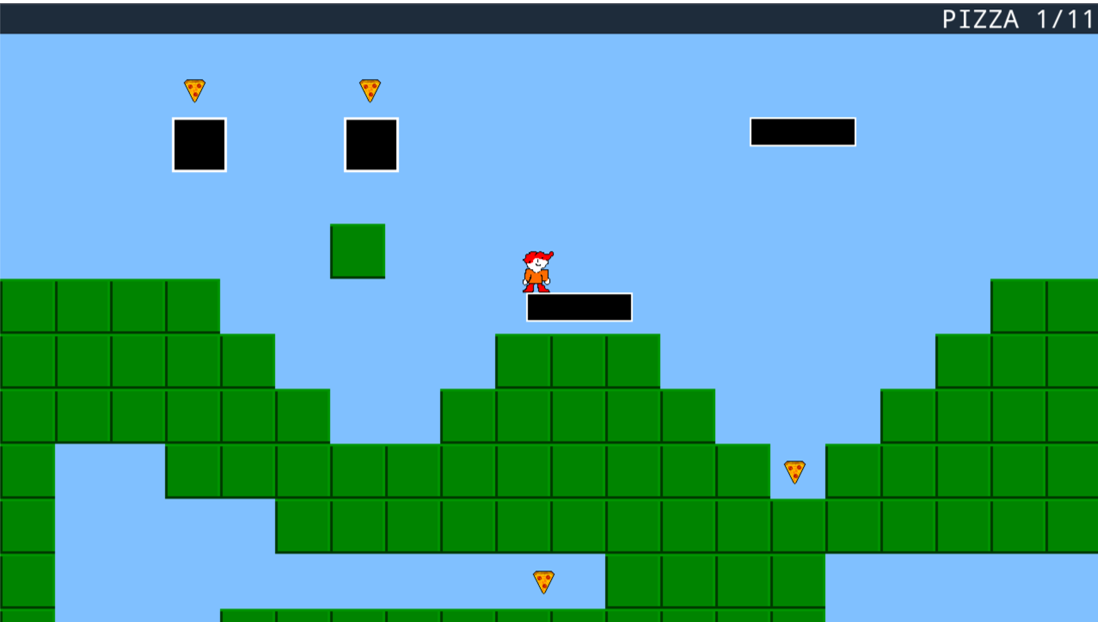
\includegraphics[height=3in]{figure1.png}
    \caption[]{Figure 1, Pete's Pizza Party: Pre-Extension}
    \label{fig:pete's pizza party}
\end{figure}


\section{Design}\label{sec:design}
Design material will be inserted here appropriately
\subsection{Flowchart}\label{sec:subsec1}

\section{Implementation and Development}


\section{Conclusion}
\cleardoublepage
\section*{References}


\end{document}
